\documentclass{beamer}

\usetheme{Warsaw}
\usecolortheme{dove}
\usefonttheme{serif}
\usepackage{tikz}
\useinnertheme{rectangles}
\useoutertheme{miniframes}
\setbeamercolor*{mini frame}{fg=black,bg=white}
\setbeamercolor{section in head/foot}{fg=black, bg=white}


% Declare lengths

\newlength{\leafnodewidth} 
\newlength{\leafnodeheightone} 
\newlength{\leafnodeheighttwo}

\newlength{\leafnodetextstart}
\newlength{\leafnodetextend}

\newlength{\internalnoderadius}

% Set length values

\setlength{\leafnodewidth}{6mm}
\setlength{\leafnodeheightone}{3mm}
\setlength{\leafnodeheighttwo}{9mm} 

\setlength{\leafnodetextstart}{10mm}
\setlength{\leafnodetextend}{13mm}

\setlength{\internalnoderadius}{3.5mm}

% Declare colors
\definecolor{leafcolorone}{RGB}{255,0,0} % Red
\definecolor{leafcolortwo}{RGB}{0,0,255} % Blue
\definecolor{internalnodecolor}{RGB}{0,255,0} % Blue


\addtobeamertemplate{navigation symbols}{}{%
	\usebeamerfont{footline}%
	\usebeamercolor[fg]{footline}%
	\hspace{1em}%
	\insertframenumber/\inserttotalframenumber
}

% Define the \leafnode command
\newcommand{\leafnode}[6]{
	\begin{tikzpicture}
		\filldraw[color=#1!90, fill=#1!3, thick, font=\tiny] (0,0) rectangle (\leafnodewidth, -\leafnodeheightone) node[midway, text=#3] {#4};
		\filldraw[color=#2!90, fill=#2!3, thick, font=\small] (0,-\leafnodeheightone) rectangle (\leafnodewidth, -\leafnodeheighttwo) node[midway, text=#3] {#5};
		\filldraw[color=white!100, fill=white!100, thick, font=\scriptsize] (0,-\leafnodetextstart) rectangle (\leafnodewidth, -\leafnodetextend) node[midway, text=#3] {#6};
	\end{tikzpicture}
}

% Define the \internalnode command with a color argument
\newcommand{\internalnode}[3]{
	\begin{tikzpicture}
		\filldraw[color=#1!90, fill=#1!5, thick, font=\scriptsize] (0,0) circle (\internalnoderadius) node[midway, text=#2] {#3};
	\end{tikzpicture}
}

\begin{document}

\begin{frame}{Tree}
	
	\tikzstyle{level 1} = [sibling distance=38mm]
	\tikzstyle{level 2} = [sibling distance=25mm]
	\tikzstyle{level 3} = [sibling distance=22mm]
	\tikzstyle{visible_edge} = [->, draw, blue, thick]
	\tikzstyle{edge from parent} = [draw, teal, thick]
	\tikzstyle{emph} = [edge from parent/.style={->,violet,draw,thick}]
	\tikzstyle{norm} = [edge from parent/.style={draw, teal, thin}]
	\tikzstyle{noedge} = [edge from parent/.style={draw, white, thin}]

	\tikzstyle{every node} = [inner sep=0]
	
	\begin{figure}
		
		\begin{tikzpicture}[
			level distance=12.5mm
			]
			%\useasboundingbox (-6.8,-6.8) rectangle (-4,-4);
			
			\node {\internalnode{green}{black}{1.00}}
			child[emph]{
				node {\internalnode{green}{black}{0.48}}
				child[emph]{
					node {\internalnode{green}{black}{0.31}}
					child[norm]{
						node {\leafnode{red}{blue}{black}{0.15}{D}{000}}
					}
					child[emph]{
						node {\leafnode{red}{blue}{black}{0.16}{E}{001}}
					}
				}
				child[norm]{
					node {\leafnode{red}{blue}{black}{0.17}{A}{01}}
				}
			}
			child[norm]{
				node {\internalnode{green}{black}{0.52}}
				child[norm]{
					node {\leafnode{red}{blue}{black}{0.17}{C}{10}}
				}
				child[norm]{
					node {\leafnode{red}{blue}{black}{0.35}{B}{11}}
				}
			};
			
		\end{tikzpicture}
		
	\end{figure}
	
	
\end{frame}


\begin{frame}{The Problem}
	\begin{block}{Range Sum Query}
		You are given an integer array $a$. Answer $q$ queries of the following form: \\
		\centering
		\begin{itemize}
			\item $sum(i, j)$ : returns $\sum_{k=i}^{j} a[k]$
		\end{itemize}
	\end{block}
	\pause
	\begin{example}
		\centering
		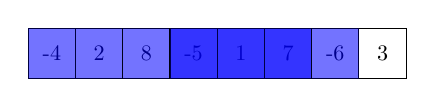
\begin{tikzpicture}[scale=0.8,transform shape]
			\onslide <2->
			\foreach \i/\j in {1/-4,2/2,3/8,4/-5,5/1,6/7,7/-6,8/3} {
				\pgfmathsetmacro\result{\i-1}
				\node[draw,rectangle, minimum width=0.75cm, minimum height=0.8cm] at (\result * 0.75,0) {\j};
			};
			\onslide <3>
			\foreach \i in {1,2,3,4,5,6} {
				\pgfmathsetmacro\result{\i-1}
				\node[draw, rectangle, minimum width=0.75cm, opacity=0.55, fill=blue, minimum height=0.8cm] at (\result * 0.75, 0){};
			};
			\onslide <4>
			\foreach \i in {4,5,6,7} {
				\pgfmathsetmacro\result{\i-1}
				\node[draw, rectangle, minimum width=0.75cm, opacity=0.55, fill=blue, minimum height=0.8cm] at (\result * 0.75, 0){};
			};
		\end{tikzpicture}
		\onslide<3-> {$sum(0, 5) = -4 + 2 + 8 + (-5) + 1 + 7 = 9$}
		\onslide<4-> {$sum(3, 6) = -5 + 1 + 7 + (-6) = -3$}
		
	\end{example}
\end{frame}

\end{document}